\documentclass[conference]{IEEEtran}
\IEEEoverridecommandlockouts
\usepackage{listings}
\usepackage{cite}
\usepackage{amsmath,amssymb,amsfonts}
\usepackage{algorithmic}
\usepackage{graphicx}
\usepackage{textcomp}
\usepackage{xcolor}
\def\BibTeX{{\rm B\kern-.05em{\sc i\kern-.025em b}\kern-.08em
T\kern-.1667em\lower.7ex\hbox{E}\kern-.125emX}}
\begin{document}

\title{Dimensionality Reduction Using Principal Component Analysis\\
{}
}

\author{\IEEEauthorblockN{Adithya Nair}
	\IEEEauthorblockA{\textit{AID23002} \\
		\textit{Amrita School Of Engineering}\\
		Bengaluru, India \\
		bl.en.u4aid23002@bl.students.amrita.edu}
	\and
	\IEEEauthorblockN{Avighna Reddy Katipally}
	\IEEEauthorblockA{\textit{AID23005} \\
		\textit{Amrita School Of Engineering}\\
		Bengaluru, India \\
		bl.en.u4aid23005@bl.students.amrita.edu}
}

\maketitle

\begin{abstract}
	Principal Component Analysis reduces the dimensionality of a set of data points by linearly projecting them onto a lower-dimensional space where the reconstruction error is as minimal as possible. This report aims to illustrate the process and its use in statistics and data visualizations.
\end{abstract}

\begin{IEEEkeywords}
	principal component analysis, statistics, mathematics
\end{IEEEkeywords}
\section{Problem Statement}
When working with data, there are times when we encounter a situation where we obtain data with a dimensionality too high to be visualized or analyzed (by dimensionality we mean the number of dimensions of the data points).

Principal Component Analysis is a method by which data points with a higher dimensionality are projected onto a linear subspace, with as minimal of a reconstruction error and projection error as possible.
\section{An Intuition For The Method}
\subsection{Projection And Reconstruction Error}
Principal Component Analysis works by projection, it takes a higher dimensional space and linearly projects them to a lower dimensional subspace, in a manner that makes sure that the reconstruction of this data gives as minimal of an error as possible.
\subsubsection{Projecting two-dimensional data to a line}

Let's say we have a set of data points in 2-dimensional space, and our goal is to place these data points in a line while mirroring their relationship to every other data point as closely as possible

Let's represent these data points as a vector \(\vec{x}\), We choose the unit vector \(\hat{v}\) (which is the unit vector that provides the least reconstruction error upon projection for \(x\)). The rest of this report deals with how to find this unit vector but assume that we have found the unit vector \(\hat{v}\) with the aforementioned property

\begin{figure}
	\centering
	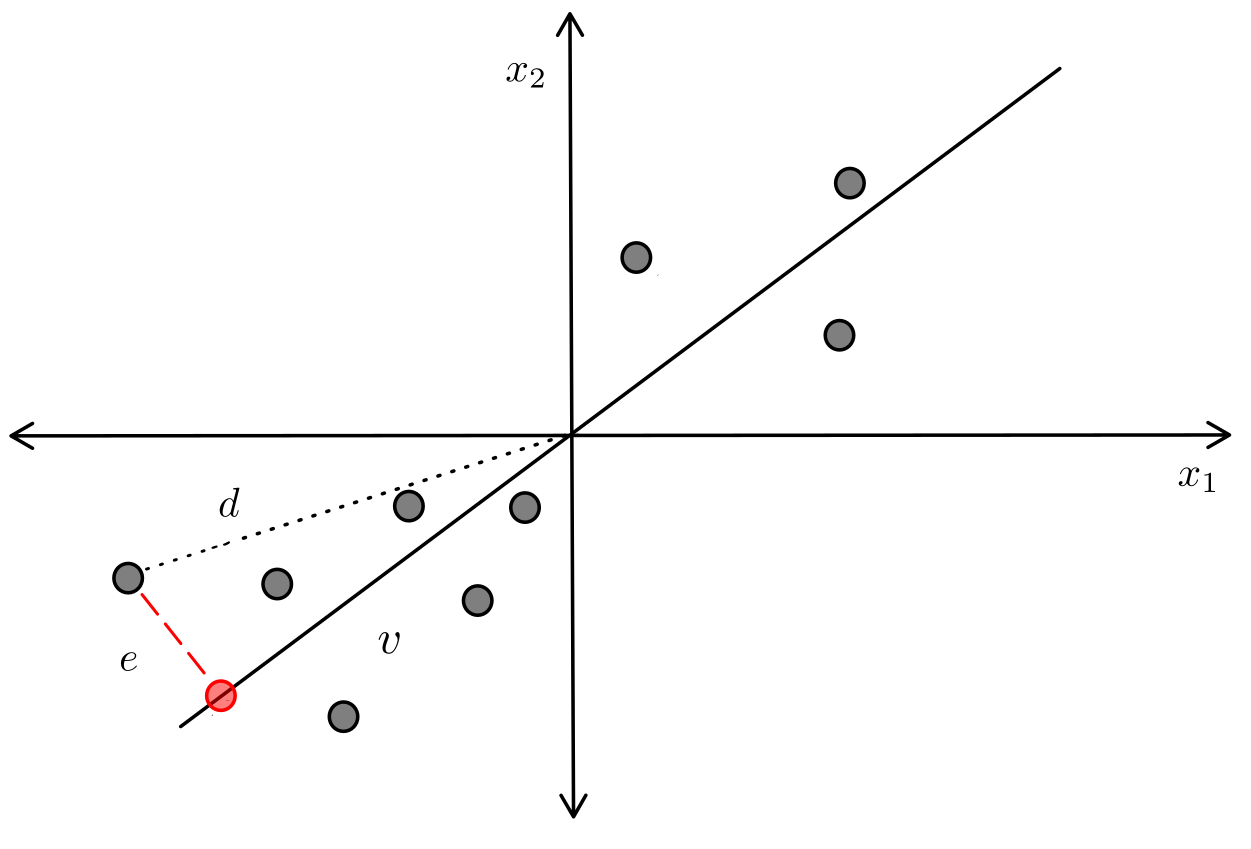
\includegraphics[width=1\linewidth] {assets/2024-08-20-Note-16-54.png}
	\caption{Projection onto a 1-dimensional subspace}
	\label{fig:enter-label}
\end{figure}

Then the projection \(x_{||}\) is done by,
$$x_{||} := (\hat{v} \cdot x) \hat{v}$$
Where \(v^Tx\) gives us the projection value and  \(v\) gives us the direction, we can write \(v^Tx\) as \(y\) to get,

$$x_{||} = y \hat{v} $$

This projection is clearly not the same as the original data points, which means that there is an error to account for between the projected points and the original data points. To compute this error, we take the mean squared distance between the projected data points and the original data points (although we can take just the distance, the squared distance is convenient for computation)

$$\text{Reconstruction Error} = \Sigma_{i = 1}^{n} \| \vec{x} - \vec{x_{||}} \|^{2}$$

Where \(n\) is the number of data points. Since we're dealing with vectors, we can write an expression for the individual components as well,

$$\text{Reconstruction Error} = \Sigma_{i = 1}^{n} \Sigma_{j=1}^{m}(x_{j} - x_{||_{j}})^{2}$$

Where \(m\) is the dimensionality of the data points.
\subsection{Reconstruction Error And Variance}

The reconstruction error here is the distance between the projected data points and the real data points. This error obviously depends on the direction we project onto. When a vector is projected, it is done orthogonally, since that is the shortest distance between the two points. This distance is the reconstruction error. The distance of the origin to the data point $d$, the distance of the origin to the projected point $v$ and the reconstruction error forms a right-angled triangle $r$

We have by Pythagoras' theorem,
$$r^2 + v^2 = d^2$$

If this is the case, we know that choosing the right direction involves making $r^2$ as low as possible. The only way to do that in the above equation is by making $v^2$ as high as possible (since the distance of the original data point to the origin will never change)

So minimizing the error, requires maximizing the distance of the projected data point from the origin.

Let's say that each data point itself has the mean subtracted from it. What this would imply is that the mean of the data is now the origin. So $v$ represents the distance from the mean of the data. We have a term for discussing the distance of a data point from the mean called variance.

Thus, we need to maximise the variance of the data to find the direction in which projecting the data has as minimal of an error as possible.

\subsection{Covariance Matrix}
Covariance is a statistical tool that maps the relationship of two random data points with each other. If a pair of data points has a positive covariance, then the data points 'vary' with each other or change in the same direction. If they have a negative covariance, then the data points don't 'change' in the same direction.

How do we determine the direction of maximal variance. We can determine the individual component variances. For a given vector $$x=(x_1, x_2)^T$$, then the variances of the first and second component can be written as $$C_{11} := \langle x_1 x_1\rangle$$ ,$$C_{12} := \langle x_1 x_2\rangle$$, (the angle brackets indicate 'averaging' over all data points)

A relatively large value of \(C_{11}\) implies that the entire set of data points varies closely in the \([1,0]^T\) unit vector direction. Similarly, for \(C_{22}\), the data points varies most along the \([0,1]^T\) direction.

In other words, the covariance matrix contains the direction of maximum variance. This is what we need to make sure the reconstruction error is minimal as shown earlier.

\subsection{PCA By Diagonalizing The Covariance Matrix}

To find the direction with which the data points vary most in, we take the covariance matrix and find the axis along which it is most varying. We diagonalize the covariance matrix by SVD. The element with the largest value corresponds to the direction that the data varies most in.

Diagonalization is done by finding the eigenvalues and eigenvectors of the matrix. The eigenvector corresponding to the largest eigenvalue is the direction which our data must be projected on to yield the least amount of reconstruction error.

\section{Implementation of Dimensionality Reduction}

Dimensionality Reduction is a procedure by which we reduce the number of variables required. We do this process to make the operations we run  less computationally intensive. Given what we know about principal component analysis and how it finds the best subspace to project data onto with the least reconstruction error, we shall demonstrate how we can reduce the dimensionality of a dataset.

\subsection{Standardization}
Standardization is used for two major reasons:
\begin{enumerate}
	\item It ensures that all the dataset's features contribute equally to the final result. Since we have numerical values, and we're working with numerical algorithms, it's best to ensure that the data itself is balanced.
	\item We're specifically using the z-score method for standardization, the dataset obtains two properties, the data's mean is 0 and it has a standard deviation of 1.
\end{enumerate}

The reason why the dataset's mean being zero is an advantage is that centers the data to the origin. The algorithm for PCA involves subtraction by the mean so we avoid an additional computation by performing a z-score normalization.

\begin{lstlisting}[breaklines]
scaler = StandardScaler()
standardized_data = scaler.fit_transform(matrix)
\end{lstlisting}

\subsection{Covariance Matrix}

We calculate the covariance matrix, and we observe that the diagonal elements of the matrix is one because we have standardized the data beforehand.
\begin{lstlisting}[breaklines]
covariance_matrix = np.cov(standardized_data, rowvar=False)
\end{lstlisting}

\subsection{Diagonalization and Principal Components Selection}

We find the eigenvalues and eigenvectors of the covariance matrix to find out the direction that the data varies most in. We select a  number of principal components, which is the number of dimensions we want our data to be reduced down to. We then select that number of the highest eigenvalues, and corresponding eigenvectors so that the data projected will yield the least amount of reconstruction error.

\subsection{Reduced Dimensional Data}

We then multiply the standardized data by the matrix of selected eigenvectors. This results in the data being represented in terms of the principal components.

Since the matrix of eigenvectors represents the directions in which the data varies the most, by multiplying the standardized data by this matrix, we project the data onto the new directions defined by these principal components.

\begin{lstlisting}[breaklines]
transformed_data = np.dot(standardized_data, eigenvectors_selected)
\end{lstlisting}

\section{Results}

We have taken a diabetes dataset with 20 columns which contains three binary valued columns and one outcome column. After removing all those columns, we have a dataset with a 16-dimensional space. We projected it onto a 6-dimensional space using principal component analysis.

Explained Variance Ratio is the ratio of each principal component to sum of all principal components. In other words, it can be said as this ratio tells us how much each principal component retains the ‘data’ of the original dimensional matrix. With the help of this ratio, we selected the number of principal components to use.

\begin{figure}
	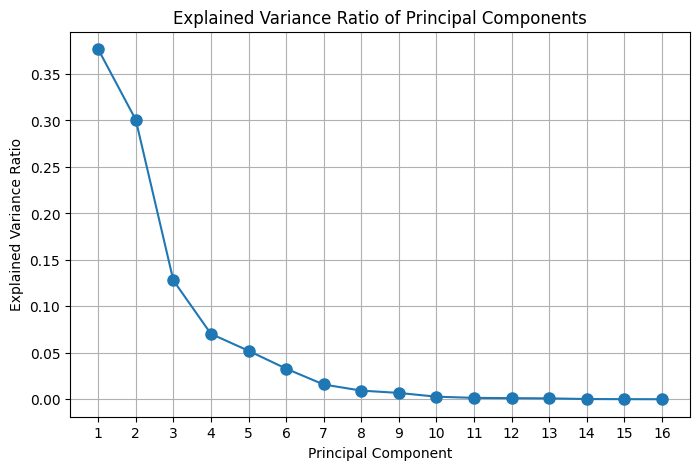
\includegraphics[width=0.4\textwidth]{assets/plot.png}
	\caption{Plot of Explained Variance Ratio}
\end{figure}

We then calculated the reconstruction error to know how the projection of 16-dimensional space onto a 6-dimensional space affects the viability of the dataset.

\begin{lstlisting}[breaklines]
reconstructed_data = np.dot(transformed_data, eigenvectors_selected.T)
error = np.mean((standardized_data - reconstructed_data) ** 2)
\end{lstlisting}

From this we get a reconstruction error of $3.9\%$, since we're using 6 dimensions, from 16 dimensions with as minimal an error as this, we have drastically reduced compute resources while still retaining the value of the dataset.

\section{Acknowledgements}
We would like to thank Ms. Sarada Jayan for providing the opportunity to research and understand this topic and its application in the field of Artificial Intelligence.

\begin{thebibliography}{00}
	\bibitem{b1} Laurenz Wiskott, ``Lecture notes on principal component analysis", Stanford: 2004, pp 2-6
	\bibitem{b2}Manjavacas, A.B. (2023) ‘Dimensionality reduction and PCA’,  Available at: https://medium.com/@anabelenmanjavacas/dimensionality-reduction-and-pca-23dbd7d6f367 (Accessed: 15 August 2023).
	\bibitem{b3} G. Strang, Introduction to linear algebra. Wellesley, Ma: Cambridge Press, 2016.
	\bibitem{b4}  G. Strang, Linear algebra and learning from data. Wellesley, Ma: Wellesley-Cambridge Press, 2019.
\end{thebibliography}
\vspace{12pt}


\end{document}
